% Set the document's formatting to "report"
\documentclass[openright]{report}

% Include titlesec[personalized chapters], graphicx[images], tocbibind[bibliography in toc], fp[variables evaluation] and glossaries/imakeidx[glossary] packages
\usepackage{titlesec}
\usepackage{graphicx}
\usepackage{tocbibind}
\usepackage[nomessages]{fp}
\usepackage[nonumberlist,acronym,toc,xindy]{glossaries}
\makeglossaries
\usepackage[xindy]{imakeidx}
\makeindex


% Edit title styling
\titleformat{\chapter}{\Huge\bfseries}{}{0pt}{\Huge}

% Set images path
\graphicspath{{../resources/images/}}

% Create uxiliary variables for worktime and version tracking 
\def \worktimeNicola {8}
\def \worktimeGiacomo {15}
\FPupn{worktimeTotal}{worktimeNicola worktimeGiacomo + 0 round}
\FPupn{version}{worktimeTotal 50 swap / 2 round}


\begin{document}

	\begin{titlepage}
		\centering

\includegraphics[width=0.50\textwidth]{polimi}\\\vspace{0.25cm}
{\scshape\LARGE Politecnico di Milano\par}\vspace{0.25cm}
{\scshape\Large Software Engineering II project: PowerEnjoy\par}\vspace{1.5cm}
{\huge\bfseries Code Inspection \par}\vspace{1cm}
{\large Gregori Giacomo and Ruaro Nicola\par}\vfill

% Bottom of the page
{\large \today \\Version \version}

	\end{titlepage}

	% Change page numbering to uppercase roman for introductory pages
    \pagenumbering{Roman}

    \tableofcontents

    \begin{abstract}
		This document provides a detailed description of the Integration Test's planning for the PowerEnJoy system. It is based on the RASD and DD documents presented in the previous deliveries and must explain to the developement team how to test the system.

	\end{abstract}

	% Change page numbering to arabic for the rest of the document
	\pagenumbering{arabic}

    \part{Requirements analysis}
    \chapter{Introduction}
    	\section{Scope of the System}
PowerEnJoy is a car-sharing service based on mobile and web applications which should allow users to reserve vehicles and use them.
\\TODO: brief architecture/algorithms/UI description
\section{Document Structure}
\begin{description} 
	\item[Introduction: ] In this chapter an introduction to the system and the Design Document is given.
	\item[Architectural Design: ] In this section an overall description of the architecture is given, it is structured into N different parts: 
		\begin{itemize}
			\item Overview: High-level components and their interaction
			\item Component view
			\item Deployment view
			\item Runtime view
			\item Component Interfaces
			\item Selected architectural styles and patterns
			\item Other design decisions
		\end{itemize}
	\item[Algorithm Design: ] In this chapter the implemented algorithms are discussed and presented using flow-charts and pseudo-code in order to ease the comprehension and focus on the functionality.
	\item[User Interface Design: ] In this section the main choices in User Interface and User Experience design are discussed.
	\item[Requirements Traceability: ] In this section a clear link between requirements specification (RASD) and design decisions (DD) is created.
\end{description}
	\chapter{Actors Identification}
	    \section{Guest}
A guest is a person that hasn't already registered to the system. She can only proceed with a new registration or log in.
\section{User}
We believe that PowerEnJoy can be used by a wide range of people that need only to access the system for benefit. A person became an user after her registration to the system, when she provides her credentials and payment information. 
\\A tipical user is a person who want to easily move around in a social end eco-friendly way. Usually she uses the service only for short travels near the \glspl{charging station}.
\\Our scope is to create an easy-to-use and efficent system that make the users satisfied and willing to use PowerEnJoy.

%\section{System}

    \chapter{Overview of the purposed system}
	    In this chapter the product and its requirements are described in order to provide a background for the "Requirements specification" part and make it easier to understand.

\section{Product perspective}
% Here we put the application into perspective with other related products, interfaces/communication means should be identified
\subsection{User interfaces} % aka "Ease of use"
\label{subsec:user_interfaces}
The user should be able to interact with the system in three ways:
\begin{itemize}
	\item{Web application}: is strongly cross-platform and then accessible from any device that can browse the web
	\item{Mobile application}: accessible from smartphones and mobile devices in order to guarantee portability and ease of use
	\item{On-Board computer}: accessible from the inside of any PowerEnjoy car, it must be extremely straightforward and let the user focus on the actual interaction
\end{itemize}
A common and friendly UI should be provided to create a sort of logical connection between the three different applications and make the user feel comfortable.

\subsection{Hardware interfaces}
The web application has no other hardware constraints despite the ones specified in subsection \ref{subsec: hw_constraints}, it should run on any device meeting such minimum requirements. Mobile application has to communicate with GPS, Antenna and WiFi modules in order to retrieve location and query the server, requirements easily met by any modern smartphone.
\\On-Board computers require a car with self-diagnostic and reporting capability.
\subsection{Software interfaces}
The web application should support devices running any modern browser while the mobile application will be developed and supported on iOS, Android and eventually WP. 
\\On-Board computer's application is device-specific and will then be designed based on the ad-hoc hardware, embedded OS and APIs.
\section{Product functions}
The system that we are to develop must let users register and then login in order to manage their account and actively access the service. The provided functionalities are clearly enumerated in section \ref{sec: proj_objectives} and here graphically described to ease the complete comprehension of the system.

\begin{figure}[!h]
	\centering
	\vspace{0.2cm}
	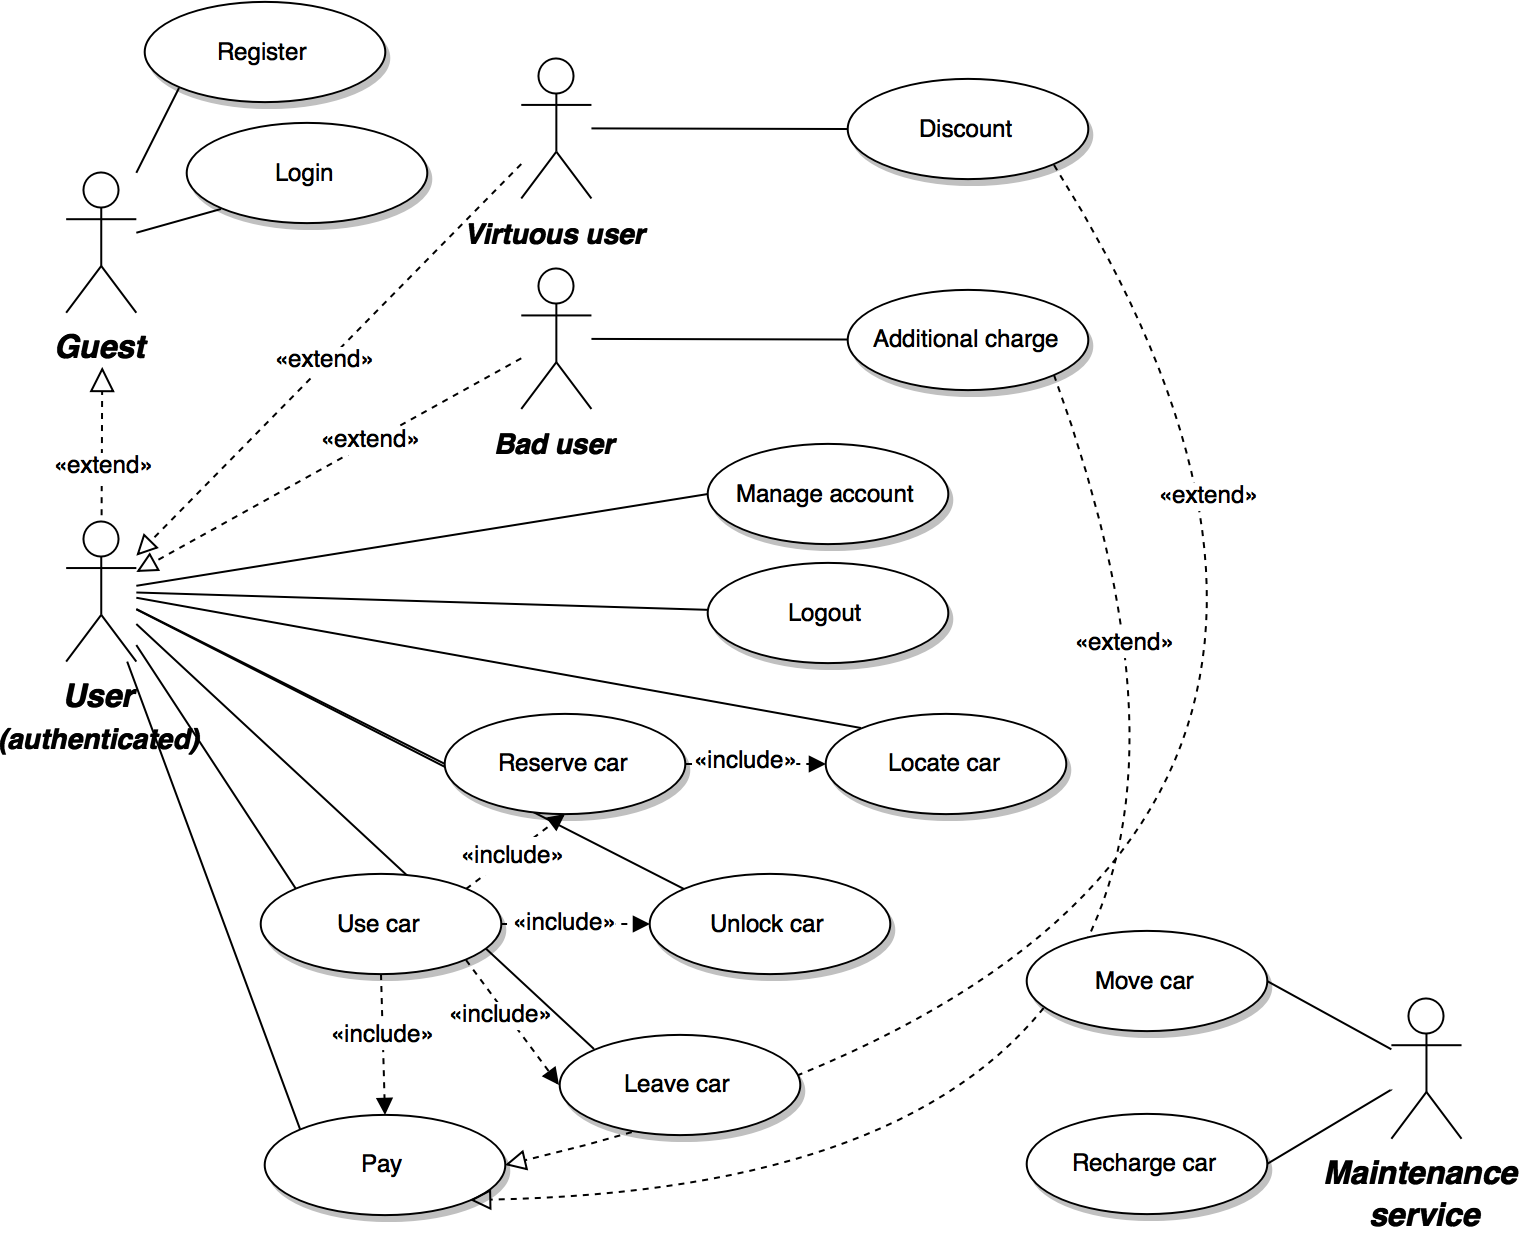
\includegraphics[width=1.0\textwidth]{/RASD/main_use_case}\\ 
	\vspace{0.5cm}
	\caption{Main use-case representing all the functionalities of the system} \label{fig:main_use_case} 
\end{figure}

\section{User characteristics}
The application should target users with a valid driving license, being at least 18 and providing a secure payment method, which must be checked before any reservation.
\\Additional legal requirements might be necessary, especially if the service is intended to spread into foreign countries
\section{Constraints}
\subsection{Regulatory policies}
Users must allow the system to collect and use personal data according to a privacy policy: data such as personal details, payment methods, transactions and locations are stored and processed in order to provide a higher service quality.
\subsection{Hardware limitations}
\label{subsec: hw_constraints}
Hardware requirements are extremely different depending on the application that is being considered; in this document, though, the on-board computer's hardware won't be discussed.
The web application development demand two main hardware constraints: 
\begin{itemize}
	\item{Stable internet connection}
	\item{Modern(supported) web browser}
\end{itemize}
The mobile application will be deployed for mobile devices, so even the memory constraints are consistents:
\begin{itemize}
	\item{ARM architecture}
	\item{At least 1GB of RAM}
	\item{At least 50MB of available storage}
	\item{Up-to-date operating system (minimum API level or OS version)} 
	\item{Stable internet connection}
	\item{GPS module may be useful but not necessary to access the service}
\end{itemize}
\subsection{Parallel operation}
The system must support heavy parallel processing because of the high number of users that are to access the service potentially at the same time.
\subsection{Reliability requirements}
The system must be opportunely reliable in order to support users while accessing the service, a 3-nines availability (\textasciitilde9hours/year) is more than enough for a non life-critical system 
\subsection{Safety and security considerations}
% todo: identify safety considerations(driving licence, safe areas, fraud, user/car damage...)
Lorem ipsum dolor sit amet, consectetur adipiscing elit, sed do eiusmod tem- por incididunt ut labore et dolore magna aliqua. Ut enim ad minim veniam, quis nostrud exercitation ullamco laboris nisi ut aliquip ex ea commodo conse- quat. Excepteur sint occaecat cupidatat non proident, sunt in culpa qui officia deserunt mollit anim id est laborum.
\section{Assumptions and dependencies}
In order for the system to work properly some domain assumptions are needed:
\begin{itemize}
	\item{Sensors and devices needed to support the functionalities of the system are already installed on vehicles}
	\item{Cars are equipped with a standard diagnostic connector and are using OBD-II communication protocols}
	\item{The GPS signal is sufficiently accurate ($\pm5m$ accuracy with A-GPS)}
\end{itemize}
% todo: complete assumptions listening to recordings and consulting notes on the firs lab
    \chapter{Functional requirements}
    	Looking at the objectives and success criteria of the project described in section 1.3, we can derive the functional requirements that PowerEnJoy have to implement. We choosed to group them by the actor involved in the function.
\begin{itemize}
\item Guest
\begin{enumerate}
	\item Registration
	\begin{itemize}
	\item She has to provide her credentials. 
	\item She has to provide her payment information.
	\item The system shall give back a password that can be used for log-in.

	\end{itemize}
	\item Log-in
	\begin{itemize}
	\item She has to provide her \gls{ID}.
	\item She has to provide her \gls{pwd}.
	%\item 

	\end{itemize}
	
	\end{enumerate}
\item User
\begin{enumerate}
	
	\item Find a car
	\begin{itemize}
	\item The system shall provide the location af all the avaible cars around the selected area.
	\item The system may know the user's location. Not necessary but useful.
	\item The system shall implement a map of the world considered.
	\end{itemize}
	
	\item Reserve a car
	\begin{itemize}
	\item The system shall kwon if a car is avaible or not.
	\item The system shall know if an user is already reserving a car.
	\item The system shall turn a car avaible or not avaible.x
	\item The system shall know the time when an user do a reservation.
	\item The system shall tag a car avaible again if a car is not picked-up within an hour from the reservation.
	\end{itemize}
	
	\item Unlock a car
	\begin{itemize}
	\item The system shall unlock a car when an user, who reaches a reserved car, tells to the system that she is nearby.
	\end{itemize}


	\item Use a car
	\begin{itemize}
	\item The system shall let each user to use only a single car at a time.
	\item The system shall start to calculate the charge as soon as the engine ignites.
	\item The system shall calculate the current cherges. The amount of money per minute is gived.
	\item The system shall notified the current charges to the user through a screen on the car.
	\end{itemize}
	
	\item Pyment
	\begin{itemize}
	\item The system shall charge the user using her payment information after each utilization.
	\item The system shall start to calculate the charge as soon as the engine ignites.
	\item The system shall stop to calculate the charge as soon as the car is parked in a safe area and the user exits the car.%same moment that the car is locked
	\item The system should apply a discount of 10\% on the last ride if it detects the user took at least two other passengers onto the car.
	\item The system should apply a discount of 20\% on the last ride if the car is left with no more than 50\% of the battery empty.
	\item The system should apply a discount of 30\% on the last ride If the car is left at special parking areas where they can be recharged and the user takes care of plugging the car into the power grid.
	\item The system should charge 30\% more n the last ride if a car is left at more then 3 KM  from the nearest power grid station or with more than 80\% of the battery empty.
	\item The system shall apply a fee of 1 EUR if a car is not picked-up within an hour from the reservation.
	\end{itemize}

	\item Lock a car
	\begin{itemize}
	\item The system shall lock the car when an user has parked the car in a safe area and the user exits the car. 
	\end{itemize}

\end{enumerate}

\end{itemize}





	\chapter{Non-Functional requirements}
    	\section{Usability}
\label{sec:usability}
 The use interface has to be user-friendly. It has to be simple, intuitive and well-organized. A typical user has not a previous knowledge of the system and we shall do it as easily to use as possible.

\section{Reliability}
The system should be avaible 24/24, 7/7, 365/365. On the other side the system has to be supported by an Internet connection that reliability depends by their providers. 
\\It should be permitted to have little stops for maintenance. If ocasionally the system has an unexpected stop however it can be accepted as the system don't cover a critical function.

\section{Performance}
The system shall support about 500000 terminals in the first implementation. At the same time the system should accept 1000 simultaneous users, and at least 90\% of the transactions should be process in less then 3 seconds.
\\The amount of information handled by the system is on the order of few Terabytes. Most of the information can be dividen into location service info, cars status info, users info and reservations info.
\\The performance will also depends by the Internet connection’s speed and reliability. In order to provide a service always available, the server should have a stable Internet connection with an adequate bandwidth.
The interactions between the user and the system has to be reduced to a minimum, in order to not overload the net. 

\section{Portability}
Our system should be very portable due to the very wide range of users. It should be compatible to all the major hardware and software components, Our mobile application should work on the most used mobile operative systems. The web application needs to be supported by all the most used browsers. The code should be developed so that only a minor part should be adapted at the specific operation system.

\section{Maintainability}
The maintainability of the system is guarantee by the administrator. The development of a 100\% bug-free software is desiderable but impossible to achive, so the administrator has to fix the system every time is needed. The administrator can also access to the data of the system for manually modify or update them.

\section{Consistency}
In order to not lose the data in case of system fault they have always to be duplicate in a backup server.  

\section{Security}
%encripted and protected by an asymmetric key and a strong hash function (e.g.: 2048 RSA key and SHA-2 hash salting)
We need to apply security protocols at different levels for ensure a correct access to the data. Each user can access to her page using her personal \gls{ID} and \gls{pwd}.
%to finish security

\section{User Interface}
As stated in section \ref{sec:usability} and subsection \ref{subsec:user_interfaces} the application's UI must be extremely friendly and functionally equivalent across devices. 
\\Regarding the mobile UI a 3-page mockup is presented (fig. \ref{fig:mobile_mockup}) to highlight the most important functions: 
\begin{itemize}
	\item{Login page: the first page presented to the end-user will obviously be a simple login/signup page where she can login using her credentials or register to the system}
	\item{Car reservation and localization: this is probably the most important use-case, the user will be able to browse and find nearby cars, eventually requesting a reservation}
	\item{Unlock: the user will request to unlock the car through a procedure similar to the one described in point 2 above, than a confirmation will be asked to provide security and force the user to really locate the car before unlocking it}
\end{itemize}
\begin{figure}[!h]
	\centering
	\vspace{0.2cm}
	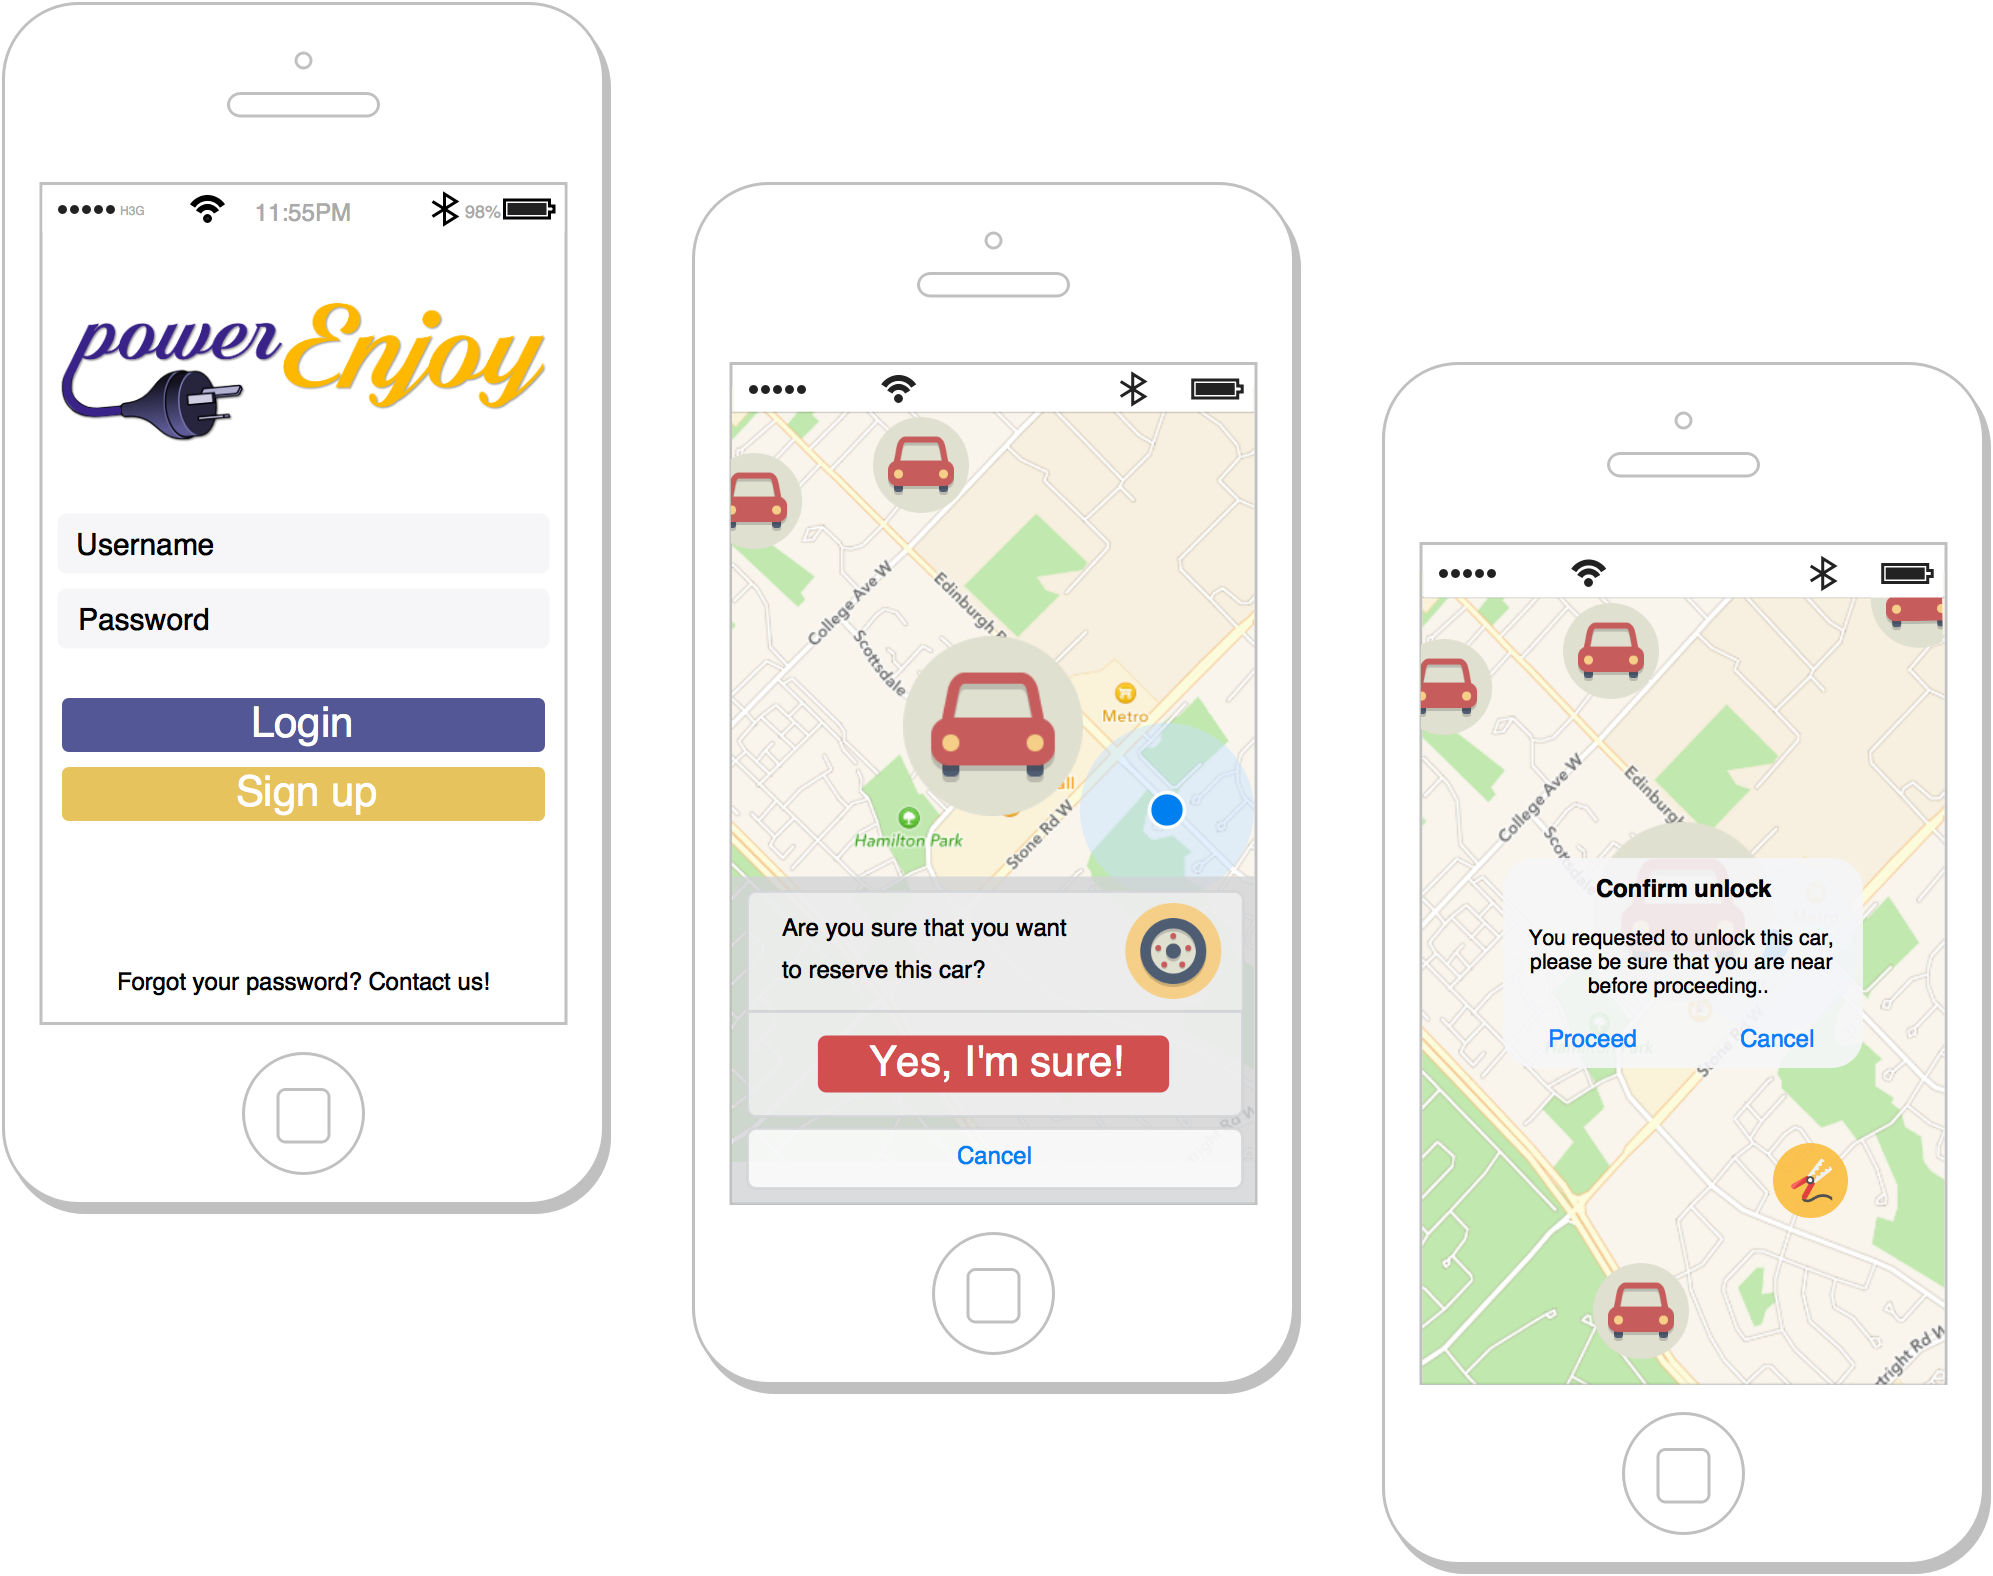
\includegraphics[width=1.0\textwidth]{/RASD/mobile_mockup}\\ 
	\vspace{0.5cm}
	\caption{3-page mockup representing the main pages of the mobile application} \label{fig:mobile_mockup} 
\end{figure}
Additional pages are the account management page, the payment page and maybe statistics related pages; those pages are not presented here as they are not strictly related to the application logic.

The web application will be really similar in features to the mobile application, the main use-cases are in fact the ones presented above in figure \ref{fig:mobile_mockup}; a basic mockup is presented (fig. \ref{fig:web_mockup}) to provide completeness:
\begin{figure}[!h]
	\centering
	\vspace{0.2cm}{}
	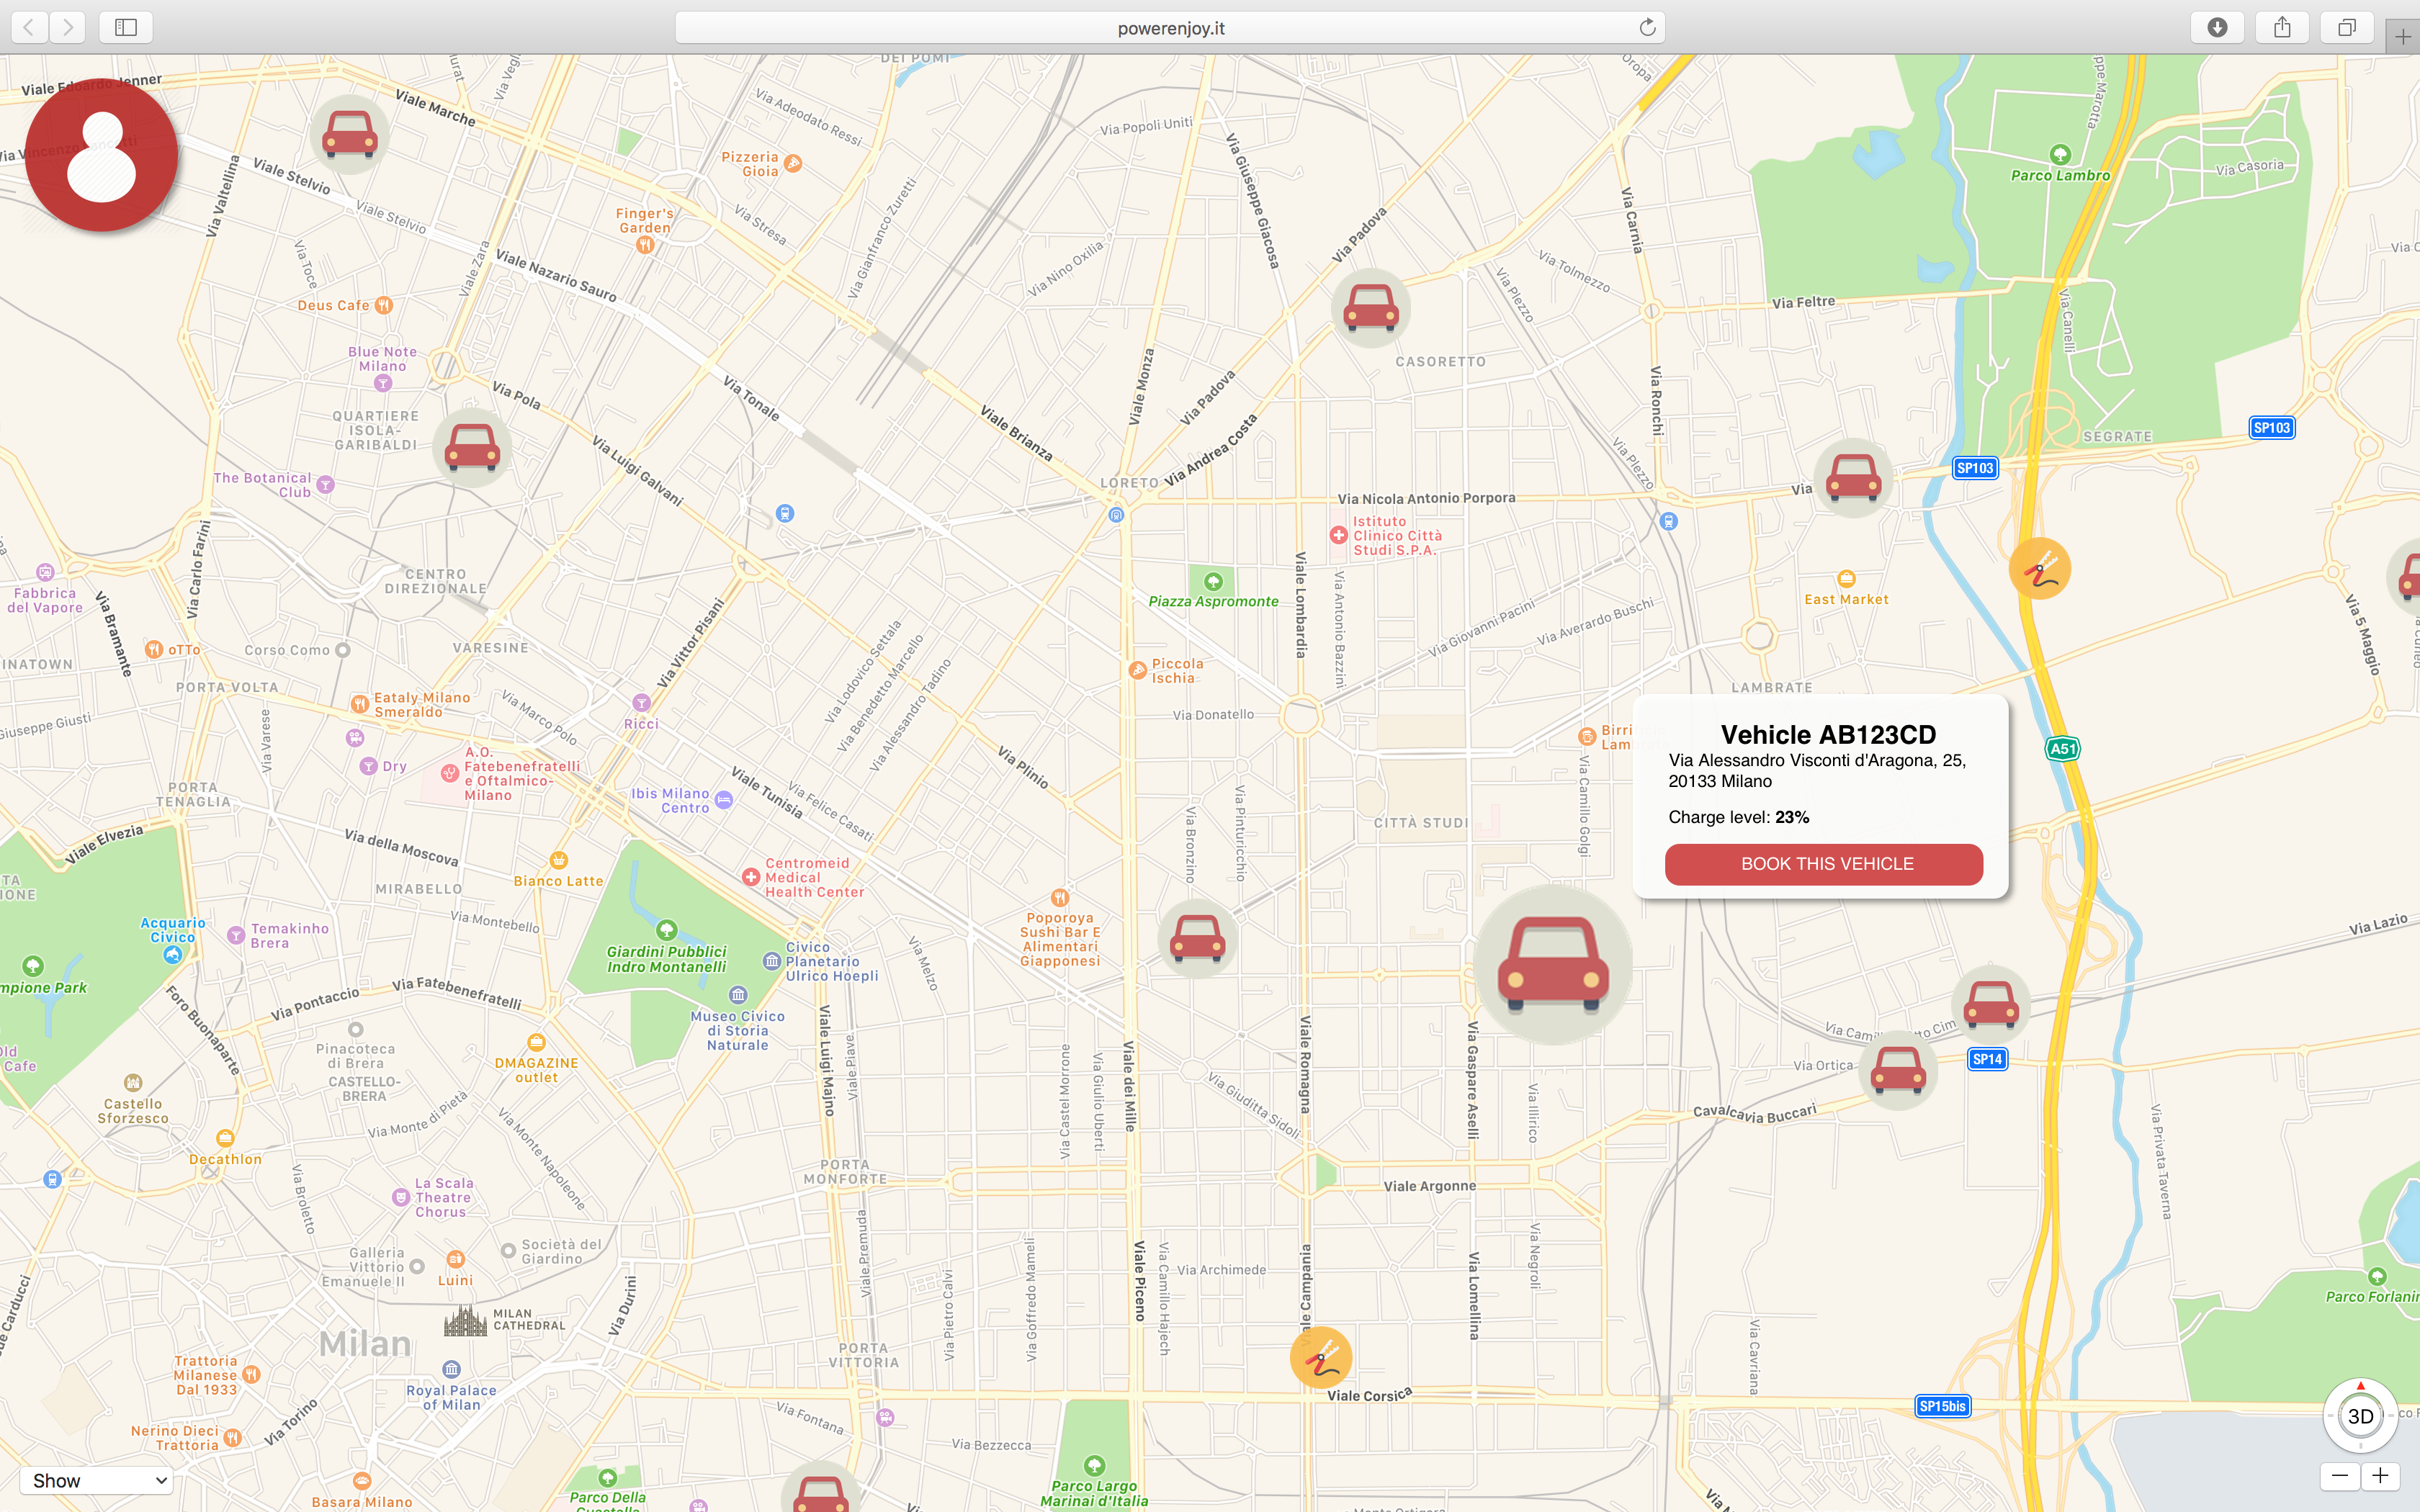
\includegraphics[width=1.0\textwidth]{/RASD/web_mockup}\\ 
	\vspace{0.5cm}
	\caption{1-page mockup representing the main page of the web application} \label{fig:web_mockup} 
\end{figure}



    % Insert a break for the table of contents
    \addtocontents{toc}{\protect\newpage}


	\part{Requirements specification}
	\chapter{Introduction}
		\section{Scope of the System}
PowerEnJoy is a car-sharing service based on mobile and web applications which should allow users to reserve vehicles and use them.
\\TODO: brief architecture/algorithms/UI description
\section{Document Structure}
\begin{description} 
	\item[Introduction: ] In this chapter an introduction to the system and the Design Document is given.
	\item[Architectural Design: ] In this section an overall description of the architecture is given, it is structured into N different parts: 
		\begin{itemize}
			\item Overview: High-level components and their interaction
			\item Component view
			\item Deployment view
			\item Runtime view
			\item Component Interfaces
			\item Selected architectural styles and patterns
			\item Other design decisions
		\end{itemize}
	\item[Algorithm Design: ] In this chapter the implemented algorithms are discussed and presented using flow-charts and pseudo-code in order to ease the comprehension and focus on the functionality.
	\item[User Interface Design: ] In this section the main choices in User Interface and User Experience design are discussed.
	\item[Requirements Traceability: ] In this section a clear link between requirements specification (RASD) and design decisions (DD) is created.
\end{description}
	\chapter{Developer Overview}
		Here a complete class diagram of our system is presented before splitting up the functionalities and provide an in-depth overview:
\begin{figure}[!ht]
	\centering
	\vspace{0.2cm}
	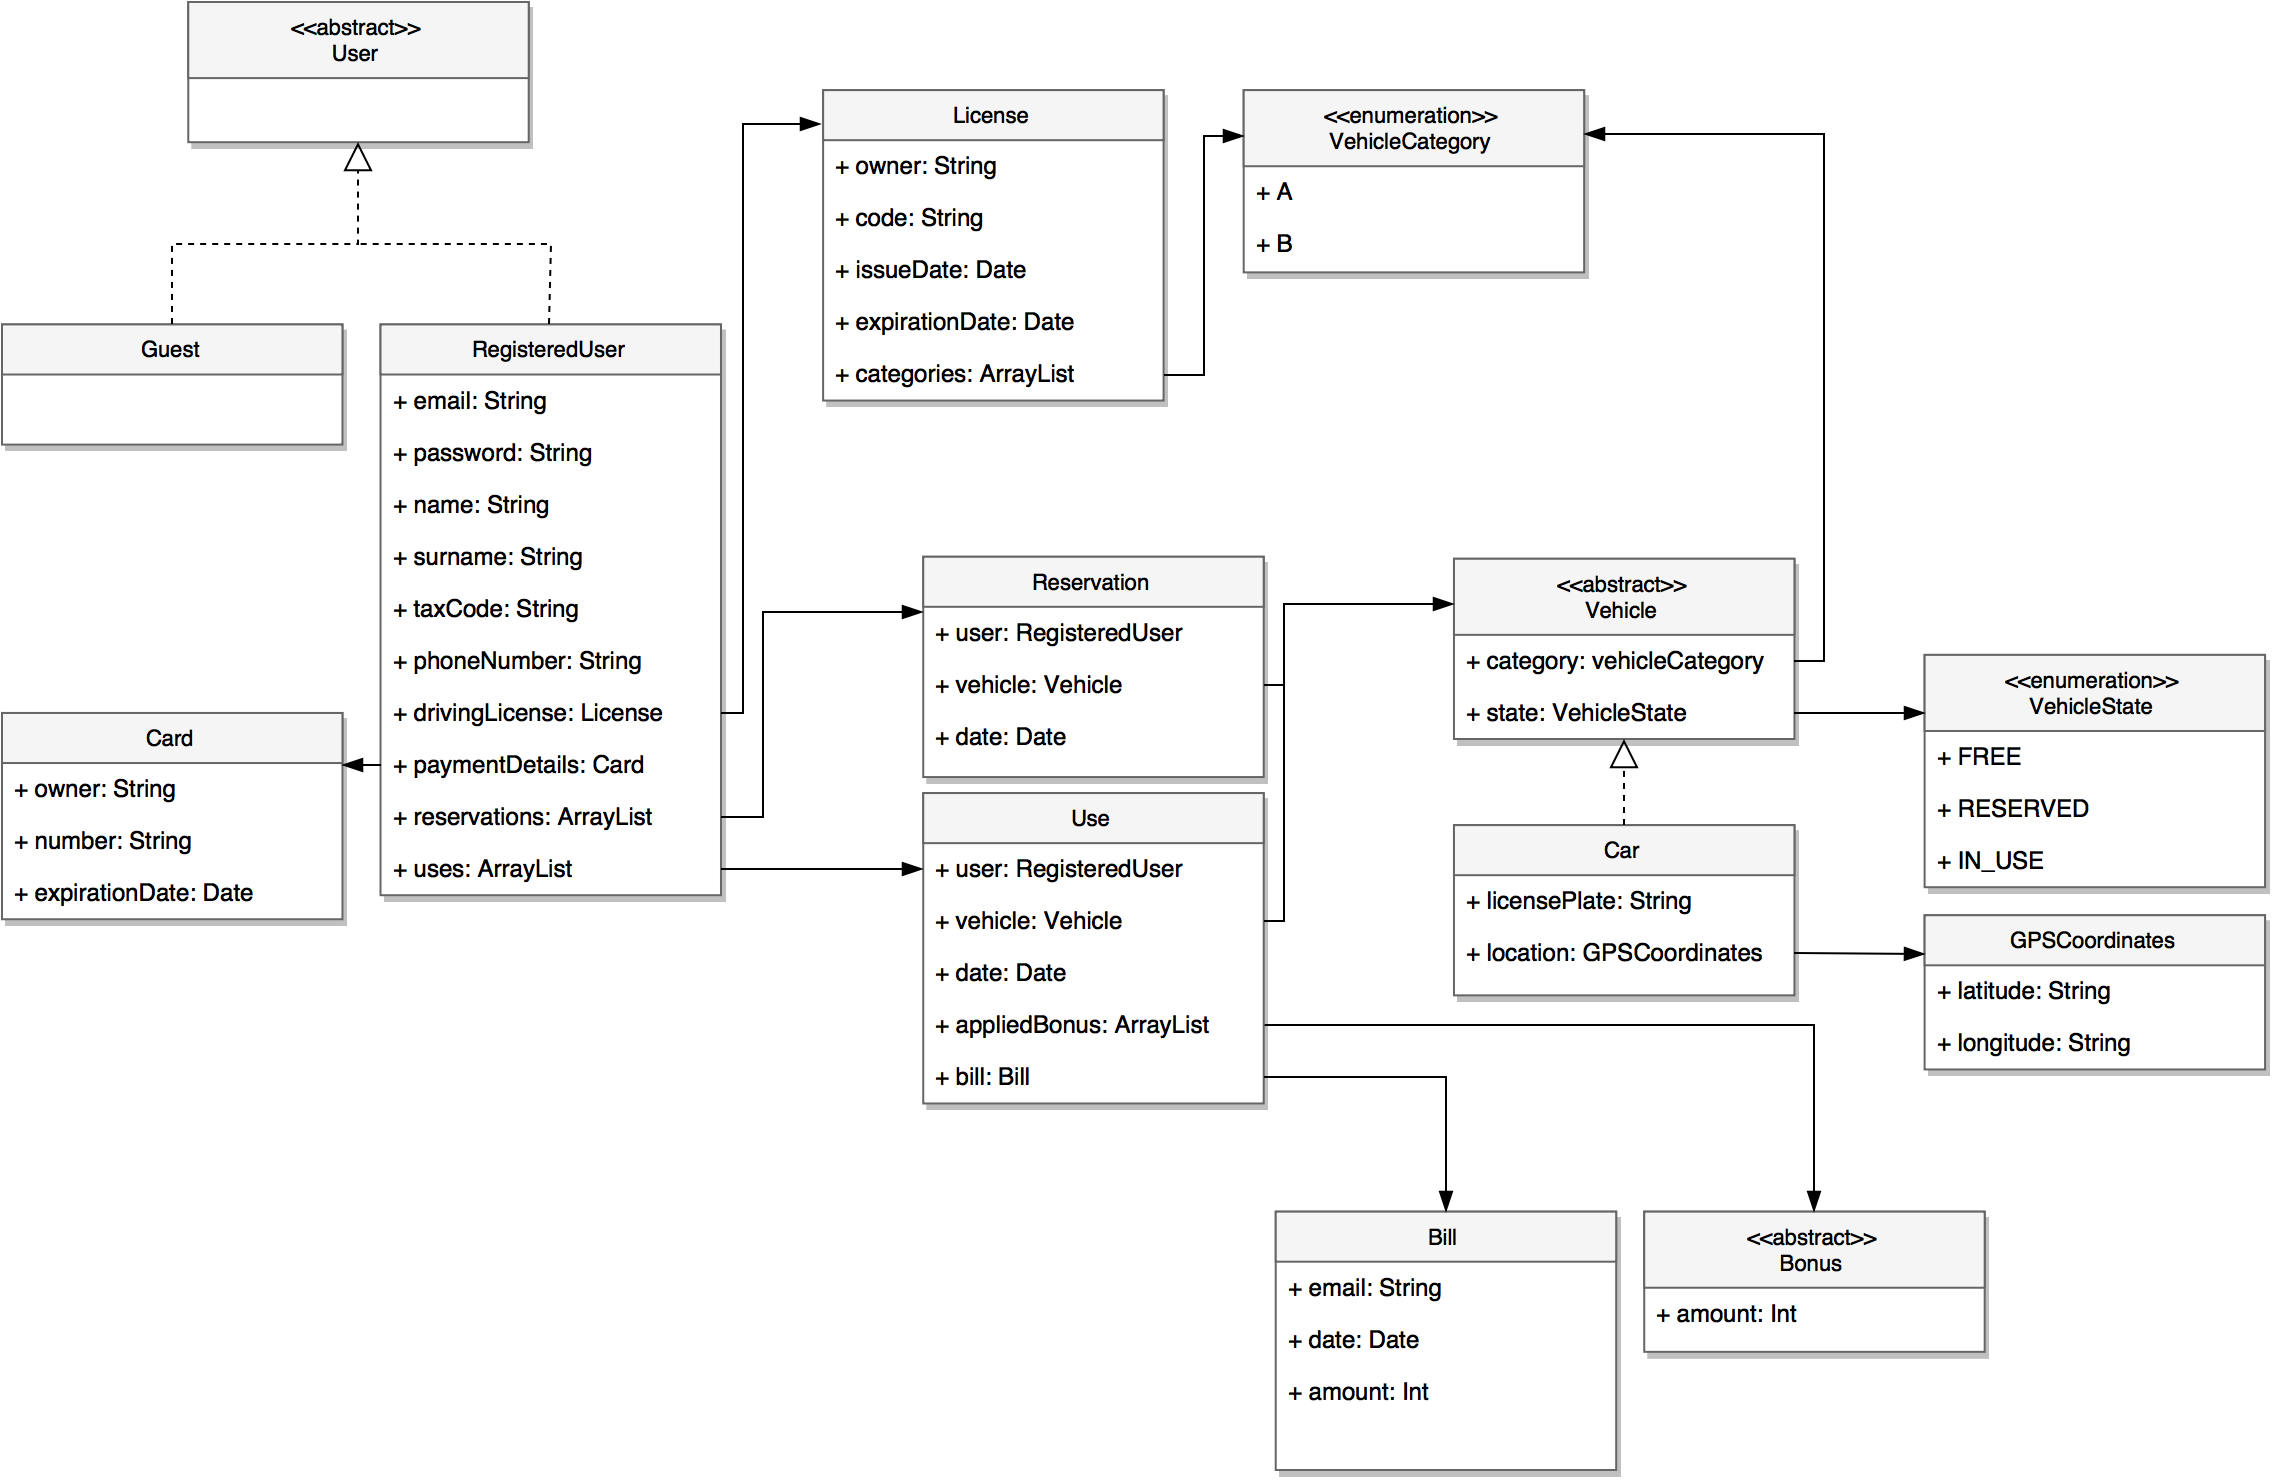
\includegraphics[width=1.0\textwidth]{/RASD/system_class_diagram}\\ 
	\vspace{0.5cm}
	\caption{Complete class diagram of the system} \label{fig:system_class_diagram} 
\end{figure}

	\chapter{System Models}
		\section{The world and the machine}

\begin{center}
	\vspace{0.2cm}
	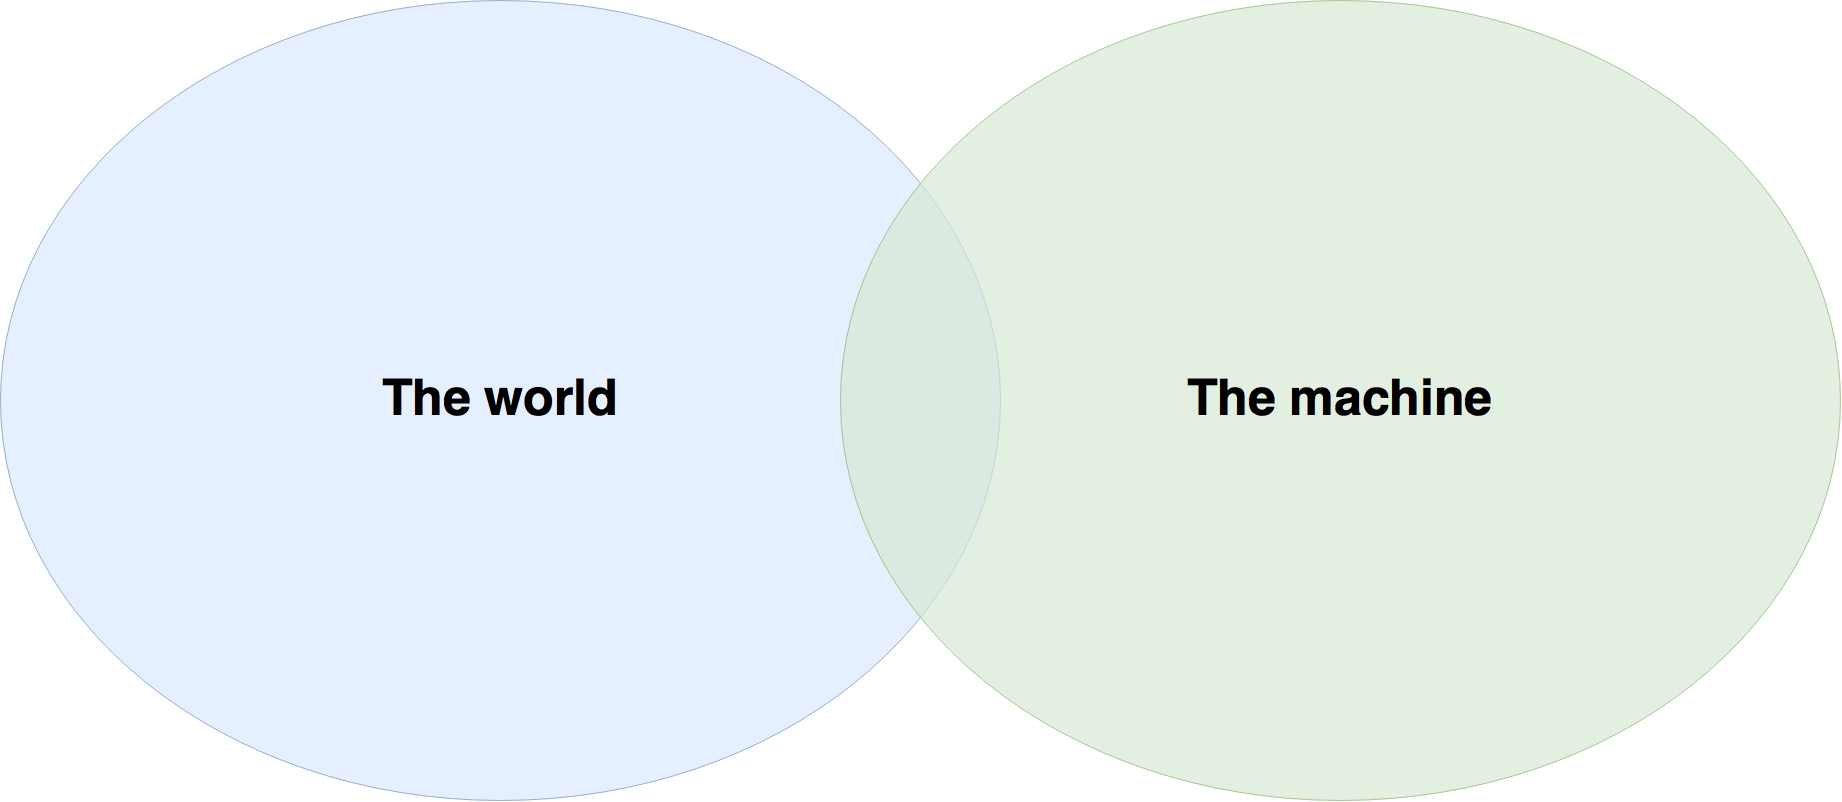
\includegraphics[width=0.50\textwidth]{/RASD/TheWorldAndTheMachine}\\ 
	\vspace{0.5cm}
\end{center}


\section{Scenarios}

\section{Use cases}


\subsection{Guest}


\subsubsection{Log-in}

\begin{center}
  \begin{tabular}{ l | p{10cm} }
    \hline
    \textbf{Name} & \textbf{Log-in} \\ \hline
    Actors & Guest\\ \hline
    Entry conditions & 
\begin{itemize}
\item The Guest has to be sucessfully registered to PowerEnJoy.
\item The Guest entres the Log-in page in the browser/ mobile application. 
\end{itemize} \\ \hline
    Flow of events &
\begin{itemize}
\item The Guest insert her \gls{ID} and \gls{pwd}.
\item The Guest clicks the Log-in button.
\item The system loads the User's homepage.
\end{itemize} \\ \hline
  	Exit conditions & The User is in the PowerEnJoy homepage. \\ \hline
	Exceptions & 
\begin{itemize}
\item The Guest provides wrong username-password pair (the system signals a LoginError).
\item The Guest doesn't fill both the fields (the systems signals an InformationLack).
\item The system is not able to complete the operation due to some internal issues or connection broken (the system signals a CennectionToSystemFail).%volendo si possono modificare i nomi delle eccezzioni.
\end{itemize} \\ \hline
  \end{tabular}
\end{center}

\subsubsection{Registration}

\begin{center}
  \begin{tabular}{ l | p{12cm} }
    \hline
    \textbf{Name} & \textbf{Registration} \\ \hline
    Actors & Guest\\ \hline
    Entry conditions & 
\begin{itemize}
\item The Guest has to have internet access.
\item The Guest entres the Sign-up page in the browser/ mobile application. 
\end{itemize} \\ \hline
    Flow of events &
\begin{itemize}
\item The Guest is shown a form to fill with her personal e-mail, name, surname, tax code and phone number. %da scegliere se l'ID viene scelto dal system o dal Guest 
\item The Guest fills the form and confirm her provided information.
\item The Guest is shown a form to fill with her drive license's information.
\item The Guest fills the form and confirm her provided information.
\item The Guest is shown a form to fill with her payment information.
\item The Guest fills the form and confirm her provided information.
\item The system sends a confirmation e-mail to the Guest's personal e-mail with an activation link.
\item The Guest clicks the link in the system's e-mail.
\item The system allocates the User in the database.
\item The system sends an e-mail to the User's e-mail with her personal \gls{pwd}.
\item The system loads the User's homepage.
\end{itemize} \\ \hline
  	Exit conditions & The Guest is registered to PowerEnJoy and became an User. Now the User is in her homepage. \\ \hline
	Exceptions & 
\begin{itemize}
\item The Guest provides an e-mail or a phone number or a tax code already used (in this case the system signals an error).
\item The Guest does not fill one or more fields in a form (in this cases the system does not allow to proceed and signals an InformationLack).
\item The Guest provided wrong payment information (in this case the system signals an error).
\item The Guest provided wrong drive license information (in this case the system signals an error).
\item The system is not able to complete the operation due to some internal issues or connection broken (the system signals a CennectionToSystemFail).%volendo si possono modificare i nomi delle eccezzioni.
\end{itemize} \\ \hline
  \end{tabular}
\end{center}
	\chapter{Alloy Modelling}
		\lstset{
    language=alloy,
    tabsize=4,
    keywordstyle=\color{alloy-keyword}\bfseries,
    commentstyle=\color{alloy-comment},
    stringstyle=\color{alloy-string},
    basicstyle=\small\fontfamily{pcr}\selectfont
}

\section{Signatures}
	\lstinputlisting{../resources/Alloy/alloy_signatures.als}

\newpage
\section{Facts}
	\lstinputlisting{../resources/Alloy/alloy_facts.als}

\newpage
\section{Predicates}
	\lstinputlisting{../resources/Alloy/alloy_predicates.als}

\section{Results}
Executing "Run show for 3" \\
Solver=sat4j Bitwidth=4 MaxSeq=3 SkolemDepth=1 Symmetry=20 \\
5642 vars. 302 primary vars. 13223 clauses. 151ms. \\
Instance found. Predicate is consistent. 49ms. \\

\newpage
\section{Generated World}
\begin{figure}[!ht]
  \centering
  \vspace{0.2cm}
  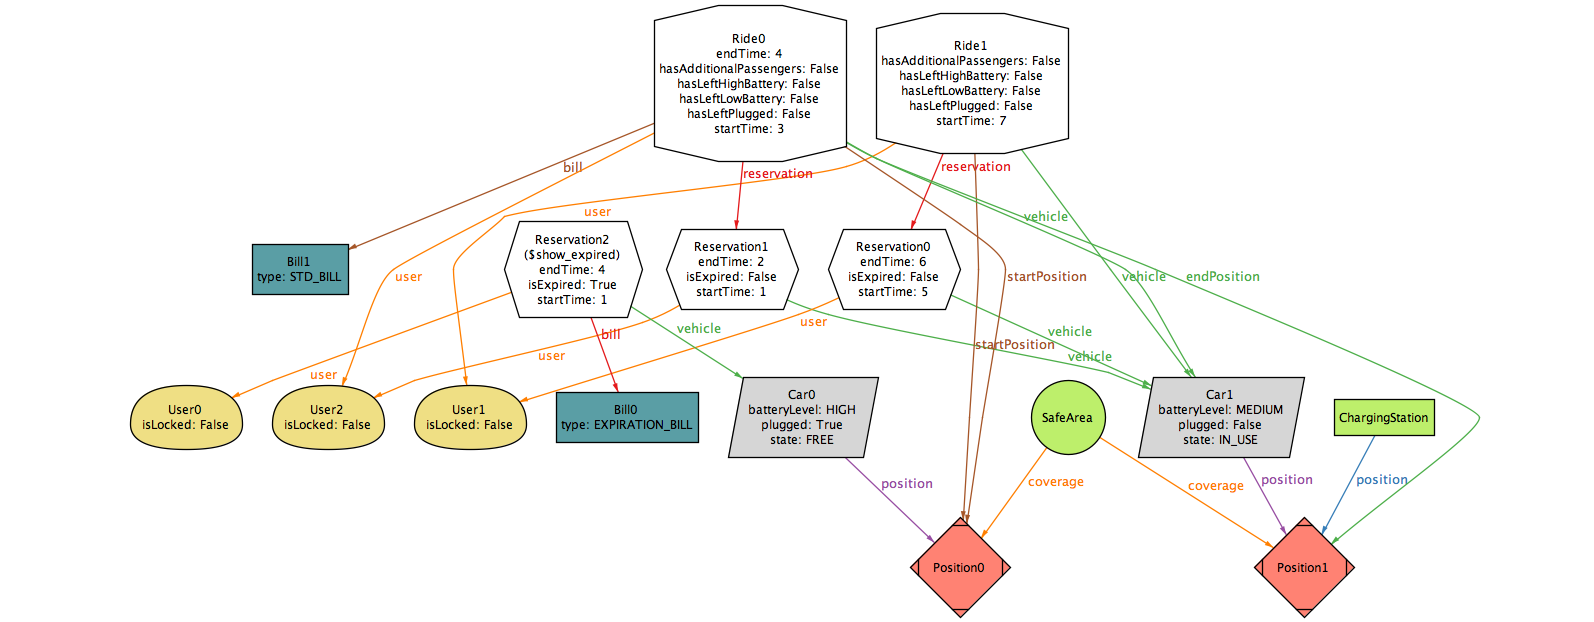
\includegraphics[width=1.4\textwidth, angle=90]{/RASD/alloy_world}\\
  \vspace{0.2cm}
  %\caption{Sequence diagram for the alloy world} 
  \label{fig:alloy_world} 
\end{figure}



	% Insert a break for the table of contents
    \addtocontents{toc}{\protect\newpage}


    \appendix
    \newpage
    \chapter{Appendix A: Used Tools}
	    \section{\LaTeX}
Used to format and redact this document
\section{\textit git}
Used as version control system in order to lead development
\section{\textit draw.io}
Used to draw mockups and diagrams
\section{\textit Alloy analyzer}
Used to analyze and verify our specification

	\newpage
	\chapter{Appendix B: Hours of work}
	    These are the hours of work spent by each group member in order to redact this document:
\begin{itemize}  
\item Ruaro Nicola: \worktimeNicola \ hours
\item Gregori Giacomo: \worktimeGiacomo \ hours
\item Total worktime: \worktimeTotal \ hours
\end{itemize}



	% Glossary entries
\newglossaryentry{charging station}
{
  name={charging station},
  description={an area used to re-charge and store electric cars},
  plural={charging stations}
}

\newglossaryentry{ID}
{
  name={ID},
  description={unique identifier associate to an user},
  plural={IDs}
}

\newglossaryentry{pwd}
{
  name={pwd},
  description={User's password, used for acess to the system},
  plural={IDs}
}

\newglossaryentry{safe area}
{
  name={safe area},
  description={Area where PowerEnJoy cars can be parked},
  plural={safe areas}
}

\newglossaryentry{reservation}
{
  name={reservation},
  description={An arrangment to secure availability of a car. An User have to reserve a car before to use it},
  plural={reservations}
}


\newglossaryentry{registration}
{
	name={registration},
	description={The act of a Guest of registering in PowerEnJoy. A Guest, after this operation, became an User},
	plural={registrations}
}
\newglossaryentry{payment}
{
	name={payment},
	description={The act of an User who is paying the system for its service. The payment information are given by the User during her \gls{registration}, they can be changed}
	plural={payments}
}
\newglossaryentry{locking}
{
	name={locking},
	description={The action of the system that automatically lock a car},
}
\newglossaryentry{un-locking}
{
	name={un-locking},
	description{The action of the system that automatically un-lock a car}
}

\newglossaryentry{car-sharing}
{
	name={car-sharing},
	description={Is a model of car rental where people rent cars for short periods of time}
}

\newglossaryentry{bill}
{
	name={payment},
	description={An amount of money that an user gives to the system for the service supplied or for fees}
	plural={bills}
}

\newglossaryentry{notify}
{
	name={notify},
	description={The act of sending a notification}
}
\newglossaryentry{notification}
{
	name={notification},
	description={A message sent by the system to an user for inform him about something important, like a reservation or a payment. It can be an e-mail, banners or messagges}
	plural={notifications}
}

\newglossaryentry{available}
{
	name={available},
	description={A car is tag available when no user is using it or has reserved it. It can also be defined free}
}
\newglossaryentry{FREE}
{
	name={free},
	description={A car is tag free when no user is using it or has reserved it. It can also be defined available}
}
\newglossaryentry{reserved}
{
	name={notification},
	description={A car is tag reserved when an user did a reservation on that car}
}

\newglossaryentry{IN USE}
{
	name={in use},
	description={A car is tag in-use when an user is using it, from the unlock to the lock of the car}
}
\newglossaryentry{OUT OF SERVICE}
{
	name={out of service},
	description={A car is tag out of service when it is parked outside a safe area or when it is left with low battery}
}
\newglossaryentry{payment information}
{
	name={payment information},
	description={Information about the way each user is going to pay the system }
}
\begin{comment}
\newglossaryentry{battery}
{
  name={battery},
  description={},
  plural={batteries}
}
\end{comment}



% Acronyms entries
\newacronym{gps}{GPS}{Global Positioning System}

	\glsaddall
	\printglossaries

	\newpage
	\begin{thebibliography}{10}
		\bibitem{sw-eng2-rules}
	Luca Mottola and Elisabetta Di Nitto, \emph{Software Engineering 2: Project goal, schedule and rules}, 2016
\bibitem{sw-eng2-ci}
	Luca Mottola and Elisabetta Di Nitto, \emph{Assignment 3: Code Inspection}, 2016
\bibitem{ofbiz}
	Apache OFBiz®, \emph{org.apache.ofbiz.service.mail.JavaMailContainer.java}, 2016
	
	\end{thebibliography}

\end{document}
